
\documentclass[useAMS,referee]{biom}
%documentclass[useAMS]{biom}
\usepackage{epsfig}
\usepackage{amsmath}
\usepackage{amsfonts}
\usepackage{float}
%\usepackage{rotating} 
\usepackage{caption}
\usepackage{subfig}
\usepackage{booktabs}
\usepackage{xspace}
%\usepackage{array}
\usepackage{enumerate}
\usepackage{enumitem}
\usepackage{titlesec}
\usepackage[figuresright]{rotating}
\setcounter{secnumdepth}{4}
\captionsetup{font=footnotesize}
\usepackage[utf8]{inputenc}
\usepackage[T1]{fontenc}  
\newcommand{\head}[1]{%
  \begin{tabular}[b]{@{}c@{}}
  #1
  \end{tabular}%
}


\author{}
\date{}
%\@addtoreset{equation}{section}
\renewcommand{\sp}{\vspace{0.2 in}}
\renewcommand{\theequation} {\arabic{section}.\arabic{equation}}
%\renewcommand{\thefigure}{\arabic{section}.\arabic{figure}}
\renewcommand{\thefootnote}{\fnsymbol{footnote}}


\def\bSig\mathbf{\Sigma}
\newcommand{\VS}{V\&S}
\newcommand{\tr}{\mbox{tr}}

\newcommand{\Bigskip}{\vspace{0.3 in}}
\newcommand{\bA}{\mbox{\bf A}}
\newcommand{\bB}{\mbox{\bf B}}
\newcommand{\bC}{\mbox{\bf C}}
\newcommand{\bD}{\mbox{\bf D}}
\newcommand{\bX}{\mbox{\bf X}}
\newcommand{\bV}{\mbox{\bf V}}
\newcommand{\bU}{\mbox{\bf U}}
\newcommand{\bW}{\mbox{\bf W}}
\newcommand{\bo}{\mbox{\bf 0}}
\newcommand{\bs}{\mbox{\bf 1}}
\newcommand{\bZ}{\mbox{\bf Z}}
\newcommand{\bY}{\mbox{\bf Y}}
\newcommand{\bR}{\mbox{\bf R}}
%\newcommand{\sbX}{\mbox{\scriptsize \bf X}}
\newcommand{\bx}{\mbox{\bf x}}
\newcommand{\by}{\mbox{\bf y}}
\newcommand{\bz}{\mbox{\bf z}}
\newcommand{\bu}{\mbox{\bf u}}
\newcommand{\ba}{\mbox{\bf a}}
\newcommand{\bc}{\mbox{\bf c}}
\newcommand{\br}{\mbox{\bf r}}
\newcommand{\bw}{\mbox{\bf w}}
\newcommand{\be}{\mbox{\bf e}}
\newcommand{\sgn}{\mbox{sgn}}
\newcommand{\epd}{\mbox{epd}}
\newcommand{\um}{\underline{\mu}}
\newcommand{\covm}{\underline{\Sigma}}
\newcommand{\sm}{\underline{\sigma}}
\newcommand{\ur}{\underline{\mbox{\bf r}}}
\newcommand{\vs}{\quad	\longleftrightarrow \quad }
\newcommand{\calF}{ {\cal F} }
\newcommand{\mle}{ {\mbox{\scriptsize MLE}} }
\newcommand{\bic}{ {\mbox{\scriptsize BIC}} }
\newcommand{\rbic}{ {\mbox{\scriptsize rBIC}} }
\newcommand{\prbic}{ {\mbox{\scriptsize prBIC}} }

\newcommand{\snr}{ {\mbox{\scriptsize SNR}} }
\newcommand{\kl}{ {\mbox{KL}} }
%\newcommand{\dim}{ {\mbox{\scriptsize dim}} }

\newcommand{\RSS}{\mbox{RSS}}
\newcommand{\sen}{\mbox{SEN}}
\newcommand{\spe}{\mbox{SPE}}
\newcommand{\wcon}{\stackrel{\cal L}{\longrightarrow}}
\newcommand{\asim}{\stackrel{a}{\sim}}
\newcommand{\var}{\mbox{var}}
\newcommand{\cov}{\mbox{cov}}
\newcommand{\id}{\mbox{id}}
\newcommand{\argmax}{\mbox{argmax}}
\newcommand{\bL}{{\bf L}}

\newcommand{\bfequiv}{\mbox{\boldmath $\equiv$}}
\newcommand{\bmu}{\mbox{\boldmath $\mu$}}
\newcommand{\bnu}{\mbox{\boldmath $\nu$}}
\newcommand{\bxi}{\mbox{\boldmath $\xi$}}
\newcommand{\btau}{\mbox{\boldmath $\tau$}}
\newcommand{\bgamma}{\mbox{\boldmath $\Gamma$}}
\newcommand{\bphi}{\mbox{\boldmath $\Phi$}}
\newcommand{\bfphi}{\mbox{\boldmath $\varphi$}}
\newcommand{\bfeta}{\mbox{\boldmath $\eta$}}
\newcommand{\bpi}{\mbox{\boldmath $\Pi$}}
\newcommand{\bequiv}{\mbox{\boldmath $\equiv$}}
\newcommand{\bvarepsilon}{\mbox{\boldmath $\varepsilon$}}
\newcommand{\btriangle}{\mbox{\boldmath $\triangle$}}
\newcommand{\bdelta}{\mbox{\boldmath $\Delta$}}
\newcommand{\beps}{\mbox{\boldmath $\epsilon$}}
\newcommand{\bepsilon}{\mbox{\boldmath $\epsilon$}}
\newcommand{\brho}{\mbox{\boldmath $\rho$}}
\newcommand{\btheta}{\mbox{\boldmath $\theta$}}
\newcommand{\bbeta}{\mbox{\boldmath $\beta$}}
\newcommand{\boldeta}{\mbox{\boldmath $\eta$}}
\newcommand{\balpha}{\mbox{\boldmath $\alpha$}}
\newcommand{\bsphi}{\mbox{\boldmath $\varphi$}}
\newcommand{\bsig}{\mbox{\boldmath $\sigma$}}
\newcommand{\bfpsi}{\mbox{\boldmath $\psi$}}
\newcommand{\bfdelta}{\mbox{\boldmath $\delta$}}
\newcommand{\bkappa}{\mbox{\boldmath $\kappa$}}
\newcommand{\bsigma}{{\bf \Sigma}}
\newcommand{\bzero}{{\bf 0}}
\newcommand{\bpsi}{\mbox{\boldmath $\Psi$}}
\newcommand{\bep}{\mbox{\boldmath $\epsilon$}}
\newcommand{\bfomega}{\mbox{\boldmath $\omega$}}
\newcommand{\bfOmega}{\mbox{\boldmath $\Omega$}}
\newcommand{\blambda}{\mbox{\boldmath $\Lambda$}}
\newcommand{\bflambda}{\mbox{\boldmath $\lambda$}}
\newcommand{\bfsigma}{\mbox{\boldmath $\sigma$}}
\newcommand{\bfpi}{{\mbox{\boldmath $\pi$}}}
\newcommand{\bupsilon}{\mbox{\boldmath $\upsilon$}}


\renewcommand{\thetable}{\Roman{table}}
\numberwithin{equation}{section}


\newcommand{\R}{\textnormal{\sffamily R}\xspace}
\newcommand{\optim}{\textnormal{\sffamily optim}\xspace}

\newcommand{\sd}{\textnormal{\sffamily Sd}\xspace}
%\newcommand{\optim}{\textnormal{\sffamily optim}\xspace}

\newcommand{\optimize}{\textnormal{\sffamily optimize}\xspace}

\def\bba{{\bf{\alpha}}}
\def\bbe{{\bf{\beta}}}
\def\bvep{\mbox{\boldmath{$\varepsilon$}}}
  \def\bv{\mbox{\bf v}}
		
\def\vep{\varepsilon}
\def\diag{\mbox{diag}}
%\def\bv{{\boldsymbol{\varepsilon}}}
\def\bb{\mbox{\boldmath{$\beta$}}}
\def\bt{\mbox{\boldmath{$\theta$}}}
\def\bpsi{\mbox{\boldmath{$\Psi$}}}

\newcommand*{\affaddr}[1]{#1} % No op here. Customize it for different styles.
\newcommand*{\affmark}[1][*]{\textsuperscript{#1}}




\title[ICES REPORT]{ICES SUMMARY REPORT}

%
%\author{%
%Author A\affmark[1], Author B\affmark[1], Author C\affmark[1], Author D\affmark[2], and Author E\affmark[2]\\
%\affaddr{\affmark[1]Department of Computer Science}\\
%\affaddr{\affmark[2]Department of Mechanical Engineering}\\
%\email{\{A,B,C,D,E\}@university.edu}\\
%\affaddr{\LaTeX\ University}%
%}


%\author
%{Natoya O. A. S. ${\mathrm{Jourdain}}^{1}$\\
% Diana J. ${\mathrm{Cole}}^{2}$,\\ %Martin S. ${\mathrm{Ridout}}^{2}$ and Marcus J ${\mathrm{Rowcliffe}}^{3}$\\
%Fisheries Dynamics, Institute of Marine Research, Nordnesgaten 50, 5005 Bergen, Norway.\\
%\emailx{jourdain.natoya@imr.no}} 


\begin{document}



\label{firstpage}

%  put the summary for your paper here

\begin{abstract}

\end{abstract}


\begin{keywords}

\end{keywords}


\maketitle

\section{NS - IBTS}

In the North Sea, the IBTS started in the 1960s as a survey that was directed at juvenile herring and was at that time called the International Young Herring Survey (IYHS). \\

\indent As it was gradually realised that the survey also yielded valuable information for other fish species, such as cod and haddock, the objectives were broadened and the survey was renamed into the International Young Fish Survey (IYFS). Besides the IYFS, which was carried out in the first quarter, a number of national surveys developed in the 1970s and 1980s that were mainly carried out in the third quarter. \\

\indent  In 1990, ICES decided to combine the international and the national surveys into the IBTS. The IBTS has been carried out twice per year (1st and 3rd quarter) since 1997, and on a quarterly basis in the period 1991-1996. \\

\indent The stratification of the survey grid has always been based on ICES statistical rectangles (one degree longitude x 0.5 degree latitude ~ 30 x 30 nautical miles). Each rectangle is usually fished by the ships of two different countries, so that at least two hauls are made per rectangle. The ICES-rectangles are used to evenly distribute the hauls over the whole North Sea (Figure \ref{0icesroufismap}).\\

\indent  Most statistical rectangles contain a number of possible tows that are deemed to be free of obstructions, and vessels are free to choose any of these positions in the rectangles that they are surveying. In some rectangles, sampling may be further stratified due to significant changes in seabed depth which may, in turn, cause variations in the fish population. \\
 
\indent   In rectangles or strata that are to be sampled more than once by the same vessel, is the IBTS manual recommends that valid hauls are separated by at least one day or by at least 10 miles wherever possible. Tows in adjacent rectangles should also be separated by at least 10 miles. \\

\indent   In practise, all countries except England (Q3) and Norway (Q1 and Q3) select the hauling position randomly from a list of clear haul positions. England and Norway use the same fixed hauls every year.  \\
  
\indent  To obtain the length distribution, the catch is sorted into species or species/sex. Where the numbers of individuals are too large for all to be measured (due to time constraints etc), a representative sub-sample is selected of at least 75 fish (although sampling a very limited length range could be adequately achieved with less). In the event that a truly representative sub-sample cannot be selected, it will be necessary to further sort the species into two or more size grades or categories (Manual for the International Bottom Trawl Surveys, version VII). \\

 \indent Otolith samples are collected within 9 specified Roundfish areas as illustrated in Figure \ref{0icesroufismap}. For all species, the same areas are used. For the target species, the following minimum sampling levels are tried to be obtained for each sampling area: \\
   
\noindent herring:  8 otoliths per 1/2 cm group \\
sprat:   16 otoliths per 1/2 cm group 8.0-11.0cm 12 otoliths per 1/2 cm group >11.0cm \\
 mackerel:  8 otoliths per 1 cm group\\
 cod:   8 otoliths per 1 cm group \\
 haddock:  8 otoliths per 1 cm group\\
 whiting:  8 otoliths per 1 cm group 
 Norway pout:  8 otoliths per 1 cm group \\
  saithe:   8 otoliths per 1 cm group \\
 
For the smallest size groups, that presumably contain only one age group, the number of otoliths per length class can be reduced. Inversely, more otoliths per length are required for the larger length classes. 



\section{The Data}


\subsection{Data type}
The International Bottom Trawl Survey (IBTS) is divided into three types and according to ICES documentation: 

\begin{itemize}
\item C types - Data calculated as catch per unit effort (CPUE) (number per hour);  
\item R types -  data by haul; and 
\item S types - sub-sampled data\\
\end{itemize}


In the HL- records the code that specifies the data is as follows:

\begin{itemize}
\item C - category catch weight is adjusted per hour;  
\item R  -  weight of the catergory catch in the haul; 
\item S  - weigth of the category catch in the subsample of the total catch.
\item If subsampling was performed per species, but the whole 
 catch was not sub-sampled, R should be reported.
\end{itemize}


\subsection{Description of specifics }

\begin{itemize}
\item CPUE - catch per unit effort
\item mCPUE - mean catch per unit effort
\item NoMeas -  Number of fish, that is, number of measured fish in the given haul or subsample, species, and sex.\\
\item HLNoAtLngt (haul number at length) - number of fish at this category in. For CPUE data should be adjusted with time. \\
\item Count - number at length per haul \\
\item TotalNo - Number of fish, that is Total number of fish in the given haul and species. \\
\item SubFactor - Factor for subsampling. Sub-sampling factor. If $1/6$ of the catch was measured, report 6.  If DataType is C, it should be reported as 1. If DataType is S,  it is always $>1$. If DataType is R, the SubFactor is = 1 or >1  for different species depending on whether they were subsampled. More details for use of SubFactor can be found in the manual.\\
\item AreaType - is sampling based on ICES statistical rectangles or  survey areas? If it's Statrecs, make sure that all CA-records  have the relevant HL-records. 0: ICES statistical Rectangles
\end{itemize}

\subsection{Species}

\begin{enumerate}

\item Pleuronectes platessa = plaice,        
\item Clupea harengus = herring  
\item Scomber scombrus = atlantic mackerel 
\item  Gadus morhua   = atlantic cod
\item Merlangius merlangus  = whiting       
\item  Trisopterus esmarkii = norway pout
\item Melanogrammus aeglefinus = haddock     
\item Sprattus sprattus = sprats 
\item Pollachius virens = saithe
\item  Scyliorhinus canicula = morgay
\item Myxine glutinosa  = hagfish  
\item  Galeus melastomus =  blackmouth catshark 

\end{enumerate}

\section{Computation of Statistics}

\subsection{Count}
\begin{itemize}
\item { Data Type R}: the Subfactor is: $a =1$ or $b > 1$. Therefore,
\begin{align}
 Count & = \mathrm{HLNoAtLngt \ \times \ Subfactor} \nonumber \\
\intertext{ or}
  Count & = \mathrm{HLNoAtLngt \times Subfactor \ a \ + \ HLNoAtLngt \times Subfactor \ b} \nonumber \\
\end{align}
 \item { Data Type C}: The Subfactor is $1$ always 
  $$ Count = \mathrm{HLNoAtLngt \Big/ \left[(Subfactor \times 60)/ Haul \ duration \right]}$$\\
  \item { Data Type S}:  HLNoAtLngt - {\bf not sure of this }\\
\end{itemize}

\subsection{Total } 
\begin{itemize}
\item { Data Type R}: the Subfactor is: $a =1$ or $b > 1$. Therefore,
\begin{align}
Total \  Number & = \mathrm{Sum(HLNoAtLngt) \times Subfactor} \nonumber \\
& = \mathrm{NoMeas \times Subfactor}  \nonumber  \\
\intertext{ or}
 Total \ Number  & = \mathrm{Sum(HLNoAtLngt) \times Subfactor \ a \ + \ Sum(HLNoAtLngt) \times Subfactor \ b} \nonumber \\
 & = \mathrm{NoMeas \times Subfactor \ a  \ + \ NoMeas \times Subfactor \ b } \nonumber  \\   
\end{align}
\item Data Type C:
$$ Total \ Number =  \mathrm{Count \Big/ (Haul \ duration  \times 60)}. $$ 
\end{itemize}

\section{IBTS Indices}
In IBTS North Sea, the indices are calculated per index area, which are specific for each species. The indices are calculated as mean at age per statistical rectangle and then as a mean of the statistical rectangles over the index area. Some statistical rectangles are reduced in size due to land or very shallow water. For herring, sprat and saithe, the mean CPUE at age are weighted with the percent covered with water depths between $10m$ and $200m$ for these statistical rectangles. 

\subsection{CPUE Per Length Class }

\subsubsection{Formulas}
\begin{enumerate}


\item The CPUE per length class per haul is computed as follows\\

\begin{itemize}
\item Data Type R: the Subfactor is: $a =1$ or $b > 1$. Therefore,
\begin{align}
 CPUE_{H,l}  & = \mathrm{(Count \ \times \ 60) \Big/ Haul \ duration} \nonumber \\
\intertext{ or}
  CPUE_{H,l} & = \mathrm{\left(Count(Subfactor \ a + Subfactor \ b) \times 60\right) \Big/ Haul \ duration} \nonumber \\
\end{align}

 \item { Data Type C}: The Subfactor is $1$ always 
  $$ CPUE_{H,l} = \mathrm{HLNoAtLngt \times  Subfactor}$$\\  
  \item Data Type S: \\
\end{itemize}


\item The mean catch per unit effort at length per statistical rectangle (ST) is defined as the sum of the number per length $(l)$  (1 cm group and 0.5 cm for herring and sprat) per haul (H) by year and quarter divided by the total hauls in the statistical rectangle, 

\begin{equation}
\mathrm{mCPUE}_{ST, l} = \frac{\sum_{ST}\mathrm{CPUE}_{H,l}}{\sum_{ST} H}
\label{mSTl}
\end{equation}

\item The mean number by index area is computed by taking the sum of the mean catch per  length (sum of $\mathrm{mCPUE}_{ST, l}$ in equation (\ref{mSTl})) in all fished rectangles divided by the number of fished rectangles in the index area, i.e.,

\begin{equation}
\mathrm{mCPUE}_{IA, l} = \frac{\sum_{IA}\mathrm{mCPUE}_{ST,l}}{\sum_{IA} ST}.
\label{mIAl}
\end{equation}

\end{enumerate}
%The final indices by length are computed by taking the sum of the mean CPUE across all statistical rectangles in round fish area divided by the number of statistical rectangles in round fish area, i.e.,
%
%\begin{equation}
%\mathrm{mCPUE}_{IA, l} = \sum_{l}\mathrm{CPUE}_{IA,l},
%\label{mIA1l}
%\end{equation}


\subsection{CPUE Per Age Class}

Age-Length-Keys (ALK) is an aggregation of individual samples from a haul combined over a larger area. For IBTS, this larger area is the Round Fish area (statistical rectangle): IBTS Area of ALK - Round fish area. \\

The CPUE per age (a), length and haul (H) is calculated as the fraction of the age distribution: 
\begin{equation}
\mathrm{CPUE}_{H, a, l} = \frac{\mathrm{CPUE}_{H,l} \times ALK_{a,l}}{ALK_{l}} 
\label{1}
\end{equation}

%There are three possibilities for obtaining age information for a length class if an age distribution is missing for that length class:

\begin{enumerate}

\item If there is no ALK for a length in the CPUE file, age information is obtained as follows: 

\begin{itemize}
\item If length class (CPUE) < minimum length class (ALK), then age=1 for the first quarter and age=0 for all other quarters (see Annex 1) \\
\item  If minimum length class (ALK) < length class (CPUE) < maximum length (ALK) then age is set to the nearest ALK. If the ALK file contains values at equal distance, a mean is taken from both values. 
\end{itemize}
\item  If length class (CPUE) > maximum length (ALK) age is set to the plus group\\
 \item  Merge ALK file with CPUE file by year, quarter, length class (see Annex 4) \\
%\item If length is less than the minimum length predefined in DATRAS, the age is set to age 1 in first quarter and 0 in all other quarters. \\
%\item Then age is set to the nearest ALK either at a length class before or at a length class after the one which misses an ALK. If there is one below and one after the length class at equal distance in length, a mean is taken. \\
% \item If the length is larger than max length, the age is set to the plus group. After the age distribution is allocated to the length distribution, the age based indices are calculated. \\
\end{enumerate}


\begin{figure}[h!]
\centering
\includegraphics[width=19cm,height=17cm,keepaspectratio]{Annex 4.jpg}
 \captionsetup{font=footnotesize, width=11cm}{
\caption{ \label{circular}ANNEX 4.}}
\end{figure}



\subsubsection{ALKRFA and CPUE: This is CPUE at age by length class (CPUEALK)} 
\begin{enumerate}
\item Merge ALKRFA and CPUE by year, quarter, RFA, length class 
\item Sum numbers at length per age per statistical rectangle
\item Sum number of hauls per statistical rectangle 
\item  Calculate mean CPUE at length per age per by statistical rectangle (=result(2)/recult(3)) 
\end{enumerate}

\subsubsection{ALKRFA and CPUE: Weighted CPUE at age by length class (CPUEALKw)- herring, sprat, saithe}
For North Sea IBTS herring, saithe and sprat, data are weighted by depth strata in the statistical rectangle (see Annex 1 and Annex 3). As herring in RFA 8 and 9 are autumn spawners, ages > 1 are set to age=0 for North Sea IBTS herring in quarter 1 in RFA 8 and 9. 

\begin{enumerate}
\item Merge ALKRFA and CPUE by year, quarter, RFA, length class  
\item Sum numbers at length per age per statistical rectangle 
\item  Sum weights of all valid hauls by statistical rectangle, following Annex 3 \item Calculate weighted mean CPUE =result(2)/result(3) 
\end{enumerate}


\begin{figure}[h!]
\centering
\includegraphics[width=22cm,height=17cm,keepaspectratio]{Annex 1.jpg}
 \captionsetup{font=footnotesize, width=11cm}{
\caption{ \label{circular}ANNEX 1.}}
\end{figure}

\begin{figure}[h!]
\centering
\includegraphics[width=22cm,height=17cm,keepaspectratio]{Annex 3.jpg}
 \captionsetup{font=footnotesize, width=11cm}{
\caption{ \label{circular}ANNEX 1.}}
\end{figure}

\subsubsection{CPUEALK: Index}
\begin{enumerate}
\item Sum CPUE per age by indexarea
\item Sum number of fished statistical rectangles in indexarea 
\item Calculate mean CPUE for the index area (=result(1)/result(2))  \\ 
\end{enumerate}
 


\subsubsection{Formulas}

The mean catch per unit effort at age per statistical rectangle (ST) is defined as the sum of the number per length $(l)$ and age $(a)$ (1 cm group and 0.5 cm for herring and sprat) per haul (H) by year and quarter divided by the total hauls in the statistical rectangle, 

\begin{equation}
\mathrm{mCPUE}_{ST, a, l} = \frac{\sum_{ST}\mathrm{CPUE}_{H,a,l}}{\sum_{ST} H}
\label{mST}
\end{equation}

The mean number by index area is computed by taking the sum of the mean catch per age and length (sum of $\mathrm{mCPUE}_{ST, a, l}$ in equation (\ref{mST})) in all fished rectangles divided by the number of fished rectangles in the index area, i.e.,

\begin{equation}
\mathrm{mCPUE}_{IA, a, l} = \frac{\sum_{IA}\mathrm{CPUE}_{ST,a,l}}{\sum_{IA} ST}.
\label{mIA}
\end{equation}

 The final indices by age are computed by taking the sum of the length classes for a given age within the index area, i.e.,

\begin{equation}
\mathrm{mCPUE}_{IA, a} = \sum_{l}\mathrm{CPUE}_{IA,a,l},
\label{mIA1}
\end{equation}





\clearpage 


\clearpage 
\section{Spatial plots for countries across year }



\begin{figure}[h!]
\centering
\includegraphics[angle=90 ,origin=c,width=19cm,height=18cm,keepaspectratio]{GFR.pdf}
 \captionsetup{font=footnotesize, width=11cm}{
\caption{ \label{circular1}Germany for the period 2004-2017.}}
\end{figure}


\begin{figure}[h!]
\centering
\includegraphics[angle=90 ,origin=c,width=19cm,height=18cm,keepaspectratio]{SWE.pdf}
\captionsetup{font=footnotesize, width=11cm}{
\caption{ \label{circular2}Sweden for the period 2004-2017.}}
\end{figure}


\begin{figure}[h!]
\centering
\includegraphics[angle=90 ,origin=c,width=19cm,height=18cm,keepaspectratio]{SCO.pdf}
\captionsetup{font=footnotesize, width=11cm}{
\caption{ \label{circular3}Scotland for the period 2004-2017.}}
\end{figure}




\begin{figure}[h!]
\centering
\includegraphics[angle=90 ,origin=c,width=19cm,height=18cm,keepaspectratio]{FRA.pdf}
\captionsetup{font=footnotesize, width=11cm}{
\caption{ \label{circular4} France for the period 2004-2017.}}
\end{figure}



\begin{figure}[h!]
\centering
\includegraphics[angle=90 ,origin=c,width=19cm,height=18cm,keepaspectratio]{NED.pdf}
\captionsetup{font=footnotesize, width=11cm}{
\caption{ \label{circular5} Netherlands for the period 2004-2017.}}
\end{figure}


\begin{figure}[h!]
\centering
\includegraphics[angle=90 ,origin=c,width=19cm,height=18cm,keepaspectratio]{NOR.pdf}
\captionsetup{font=footnotesize, width=11cm}{
\caption{ \label{circular6} Norway for the period 2004-2017.}}
\end{figure}


\begin{figure}[h!]
\centering
\includegraphics[angle=90 ,origin=c,width=14cm]{DEN.pdf}
\captionsetup{font=footnotesize, width=11cm}{
\caption{ \label{circular7} Denmark for the period 2004-2017.}}
\end{figure}



\begin{figure}[h!]
\centering
\includegraphics[angle=90 ,origin=c,width=14cm]{ENG.pdf}
\captionsetup{font=footnotesize, width=11cm}{
\caption{ \label{circular8} England for the period 2004-2017.}}
\end{figure}


\begin{figure}[h!]\label{icessurmap}
  \centering
 {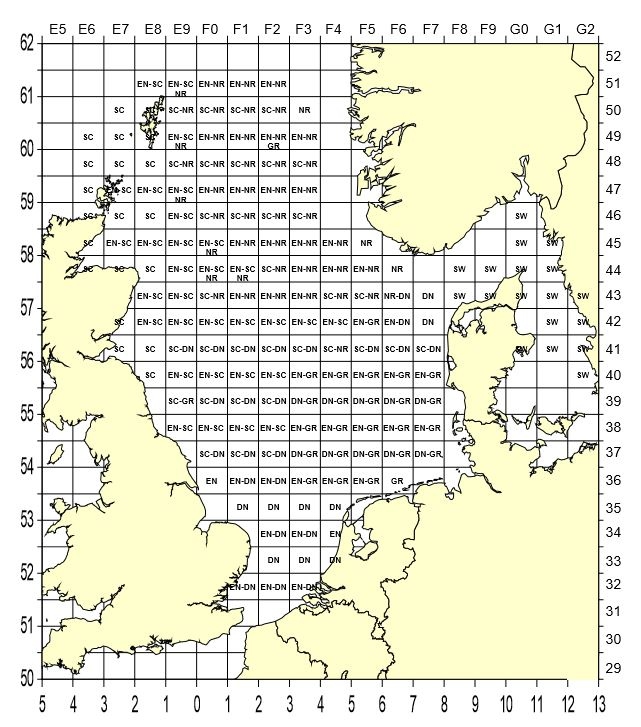
\includegraphics[width=17cm]{icessurveymap.jpg}}   
 \captionsetup{font= footnotesize, width=15cm}{
 \caption{IBTS Quarter 3 Proposed Survey Grid for all participants: D: Denmark, E: England, G: Germany, N: Norway, SC: Scotland, SW: Sweden. The country named first in the rectangle was to take the standard 30-min tow, whereas the second country could take the 15-min tow. England took only 30-min tows, therefore, all countries sharing rectangle with England took the 15-min tow.}}
\end{figure}

\clearpage
%\subsection{ICES SURVEY MAP FOR STANDARD ROUNDFISH AREAS (RFA) }
%\label{sensors1}

\begin{figure}[h!]\label{icesroufismap}
  \centering
 {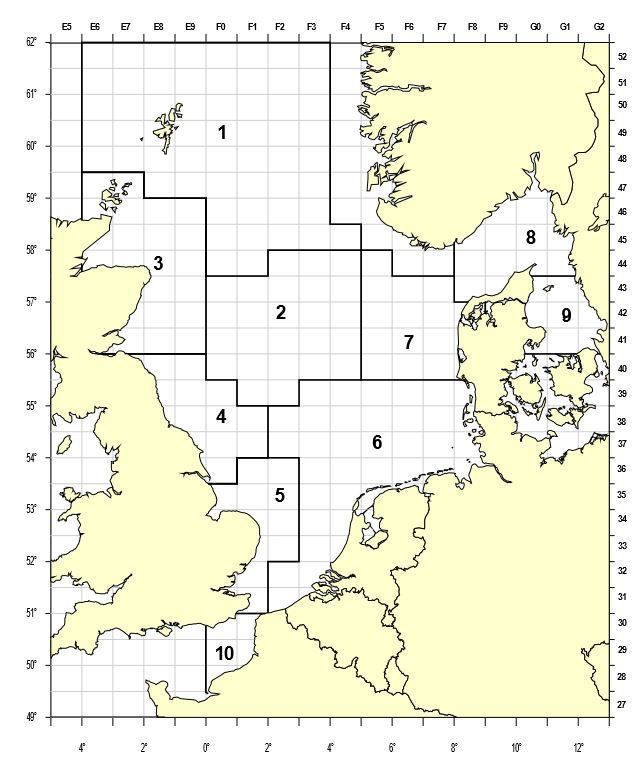
\includegraphics[width=17cm]{icesroundfishmap.jpg}}   
 \captionsetup{font= footnotesize, width=15cm}{
 \caption{Standard Roundfish Areas: used for roundfish since 1980, for all standard species since 1991. Additional RFA 10 added in 2009. For example, the number 1 indicates ICES Index Area 1, and an ICES Statitical rectangle (ST) in IA 1 is 43F1.}}
\end{figure}


 \bibliographystyle{biom} 
 \bibliography{mybibilo.bib}

%\bibliographystyle{apalike} % or try abbrvnat or unsrtnat
%\nobibliography{refs} % refers to example.bib


%\end{appendices}

\end{document}